\begin{answer}
\begin{figure}[H]
    \centering
    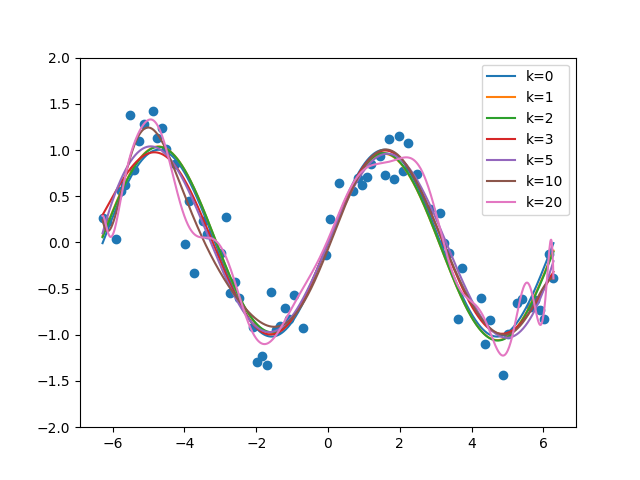
\includegraphics[width=9cm]{featuremaps/sine.png}
\end{figure}
Here we see that the polynomial terms seem to be redundant and that $sin(x)$ alone can model the data. The higher degree polynomial terms only contribute to overfitting.
\end{answer}
